\chapter{Experimentos Realizados}
\thispagestyle{plain}
\label{cap:experimentos}
\graphicspath{{./Cap4_Experimentos_Realizados/Figures/}}

A realização dos experimentos baseou-se na utilização da ferramenta de parametrização e obtenção de métricas, aplicado nas imagens tratadas de cada cena, conforme variaçoes definidas no Capítulo anterior. Os dados obtidos foram organizados de forma a facilitar a análise e comparação entre as variaçoes em cada cena e também entre os diferentes dispositivos sendo testados.

Para cada variação de resolução, que depende de uma nova seleção de parâmetros, será exibido a matriz de resultados final juntamente com as faces detectadas, após já feita a análise para se chegar a um melhor resultado, indicando quais foram os parâmetros definidos.

\section{Cena 1}

\subsection{Otimização de parâmetros}

Primeiramente, foi realizada a otimização dos parâmetros para cada variação de resolução, a partir das imagens com todas as faces disponíveis de cada resolução. No caso desta cena, que exige relativamente muito mais processamento, utilizou-se o Raspberry Pi 4B para a definição dos parâmetros, repetindo-os nos testes com o Raspberry Pi Zero W para base de comparação.

A definição dos parâmetros 'ótimos' não é objetiva. Para esta cena, buscou-se um melhor resultado em que houvesse a maior quantidade de faces detectadas com o mínimo ou nenhuma presença de falsos positivos e no menor tempo. Durante a análise, teve-se a razoabilidade de considerar na comparação entre os diferentes resultados da matriz que, um grande aumento no tempo de detecção não justifica um pequeno ganho relativo na quantidade de faces detectadas.

As próximas três subsubseções \ref{sssec:resolution1-1}, \ref{sssec:resolution1-2} e \ref{sssec:resolution1-3} mostram através de imagens, para cada resolução testada, a última iteração da matriz de resultados com os dados entrada, a célula destacada com os parâmetros escolhidos e a imagem com a faces detectadas, nos testes feitos com o Raspberry Pi 4B. 

Os parâmetros definidos de cada resolução foram usados para obter as métricas de cada variação de quantidade de faces detectáveis, e em ambos os dispositivos testados. Não será apresentado nesse documento cada resultado das métricas obtidos em tela. Todos os dados obtidos foram tabelados e utilizados para as comparações feitas nas subseções seguintes. Uma tabela resumida com esses dados é exibida no final de cada uma das próximas três subseções.


\subsubsection{Resolução 1440p} \label{sssec:resolution1-1}

Para essa resolução de 1440 x 2560 conseguiu-se chegar a uma quantidade muito boa de faces detectadas, mesmo as faces menores, de pessoas mais distantes, quase totalizando a quantidade de faces presentes na imagem. Como é normal, algumas faces não foram detectadas devido a algum adereço como chapéu, posição da face e outros possíveis fatores. Nesse caso, nenhum falso positivo foi detectado.

Parâmetros definidos: 
\begin{itemize}
    \item Min. Size Face: 0.8\%
    \item Scale Factor: 1.069
    \item Min. Neighbors: 3
\end{itemize}

\begin{figure}[H]
    \centering
    \caption[Otimização Cena 1 - resolução 1440p.]{Otimização Cena1 resolução 1440p.}
    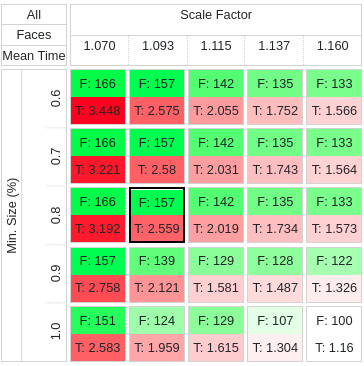
\includegraphics[width=0.70\textwidth]{Cap4_Experimentos_Realizados/Figures/cena1_param_1440p_matriz.jpg}
    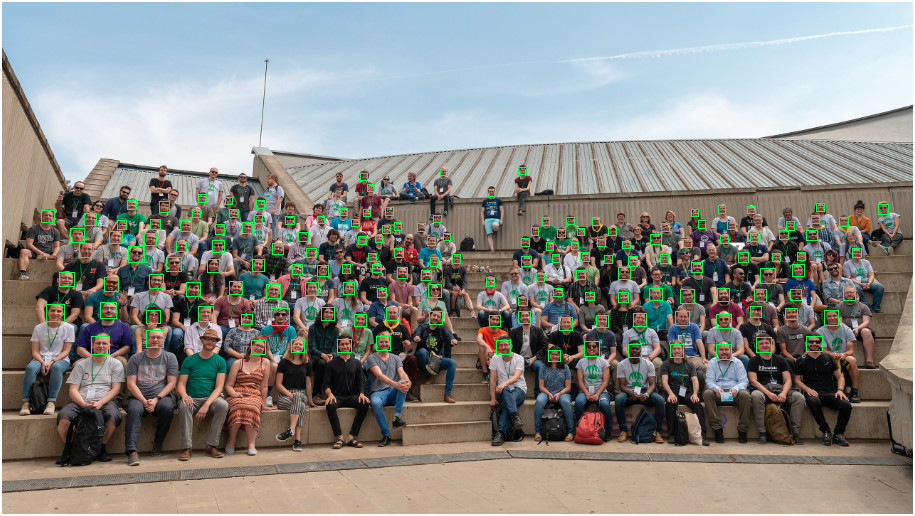
\includegraphics[width=0.85\textwidth]{Cap4_Experimentos_Realizados/Figures/cena1_param_1440p_faces.jpg}
    \caption*{Fonte: autor.}
    \label{fig:otimizacaoCena1_1440p}
\end{figure}
    
\begin{table}
    \centering
    \caption[Dados obtidos - resolução 1440p.]{Dados obtidos - resolução 1440p.}
    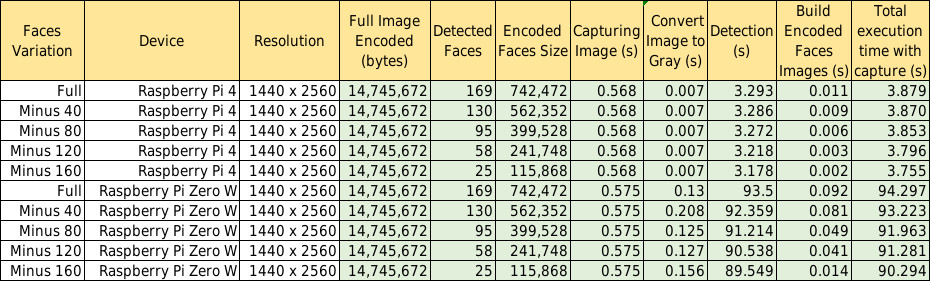
\includegraphics[width=0.90\textwidth]{Cap4_Experimentos_Realizados/Figures/cena1_dados_1440p.jpg}
    \caption*{Fonte: autor.}
    \label{fig:dadosCena1_1440p}
\end{table}

\subsubsection{Resolução 1080p} \label{sssec:resolution1-2}

Nessa resolução de 1080 x 1920, algumas faces menores começam a não serem mais detectadas, mas a quantidade de faces detectadas é relativamente grande se comparado à quantidade de faces presentes na imagem.

Observa-se uma diminuição no valor do parâmetro scale factor (que significa mais passos no escalonamento da imagem) para se obter quantidades maiores de faces detectadas e um aumento no do parâmetro min. size, já que as faces menores começam a ficar indetectáveis.

Dessa vez percebe-se a presença de alguns falsos positivos. Testou-se a variação do parâmetro min. neighbors, porém não houve melhoria.

Parâmetros definidos: 
\begin{itemize}
    \item Min. Size Face: 1.0\%
    \item Scale Factor: 1.039
    \item Min. Neighbors: 3
\end{itemize}

\begin{figure}[H]
    \centering
    \caption[Otimização Cena 1 - resolução 1080p.]{Otimização Cena1 resolução 1080p.}
    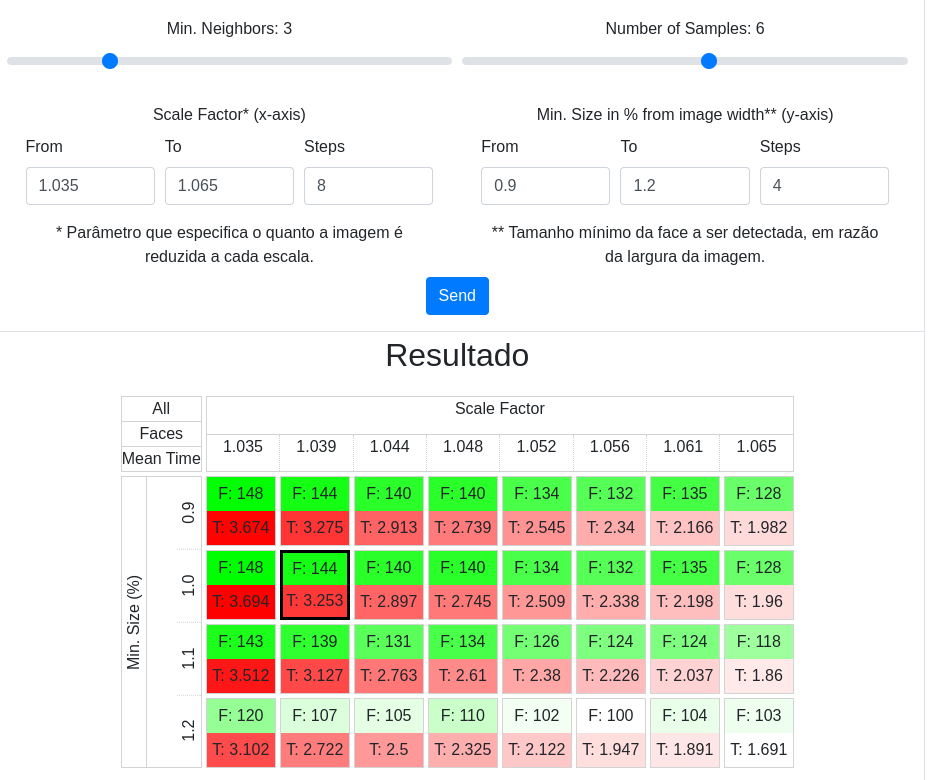
\includegraphics[width=0.70\textwidth]{Cap4_Experimentos_Realizados/Figures/cena1_param_1080p_matriz.jpg}
    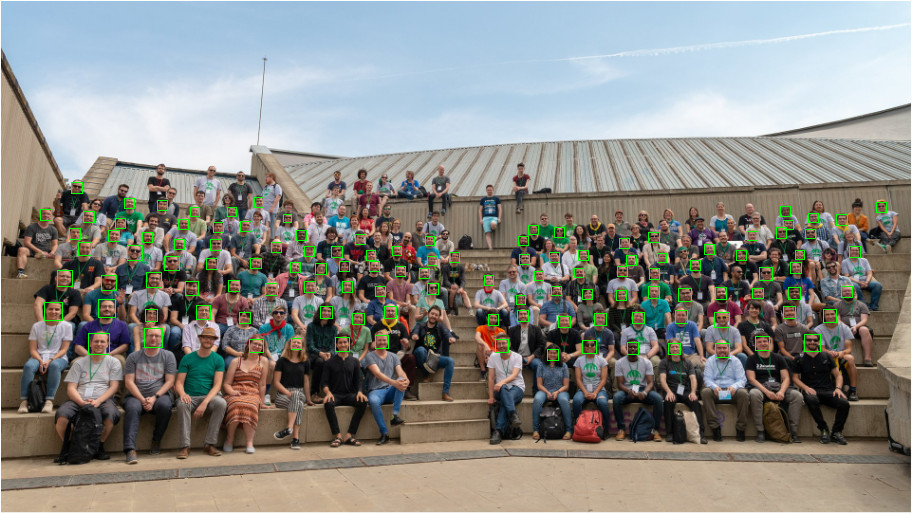
\includegraphics[width=0.85\textwidth]{Cap4_Experimentos_Realizados/Figures/cena1_param_1080p_faces.jpg}
    \caption*{Fonte: autor.}
    \label{fig:otimizacaoCena1_1080p}
\end{figure}

\begin{table}
    \centering
    \caption[Dados obtidos - resolução 1080p.]{Dados obtidos - resolução 1080p.}
    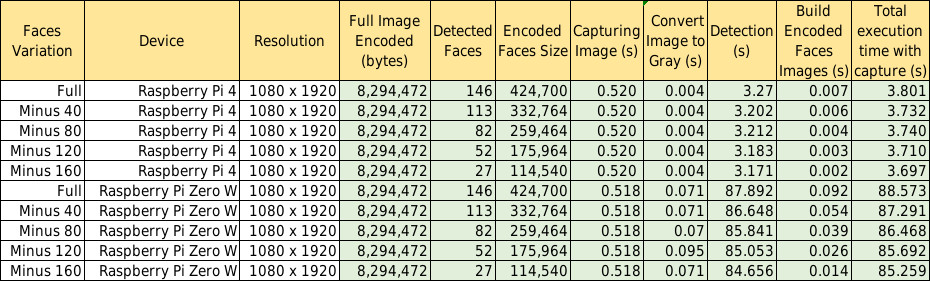
\includegraphics[width=0.90\textwidth]{Cap4_Experimentos_Realizados/Figures/cena1_dados_1080p.jpg}
    \caption*{Fonte: autor.}
    \label{fig:dadosCena1_1080p}
\end{table}

\subsubsection{Resolução 720p} \label{sssec:resolution1-3}

Nessa resolução de 720 x 1280, a queda na quantidade de faces detectadas já se torna bem considerável se comparando às resoluções maiores, sendo menos de um terço da quantidade de faces presente na imagem. Novamente, observa-se a diminuição do parâmetro de scale factor e aumento do parâmetro min. size, devido às faces menores não detectáveis.
Também percebe-se a presença de falso positivo. Testou-se também a variação do parâmetro min. neighbors. Aumentando-se de 3 para 4, observou-se a redução de falsos positivos.

Parâmetros definidos: 
\begin{itemize}
    \item Min. Size Face: 1.6\%
    \item Scale Factor: 1.024
    \item Min. Neighbors: 4
\end{itemize}

\begin{figure}[H]
    \centering
    \caption[Otimização Cena 1 - resolução 720p.]{Otimização Cena 1 - resolução 720p.}
    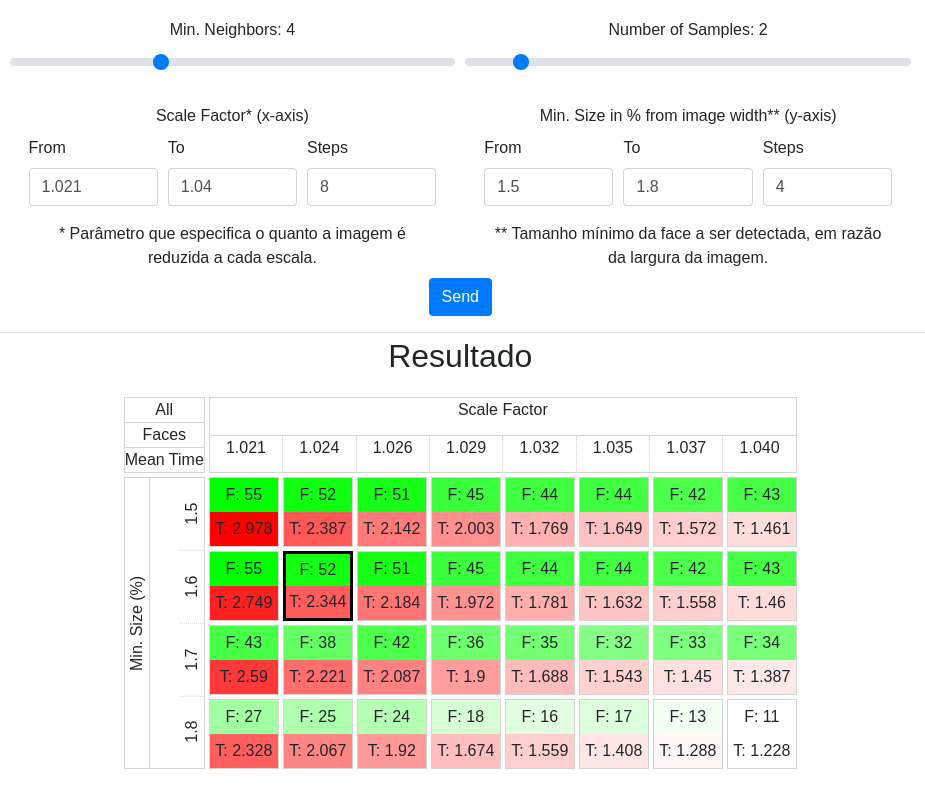
\includegraphics[width=0.70\textwidth]{Cap4_Experimentos_Realizados/Figures/cena1_param_720p_matriz.jpg}
    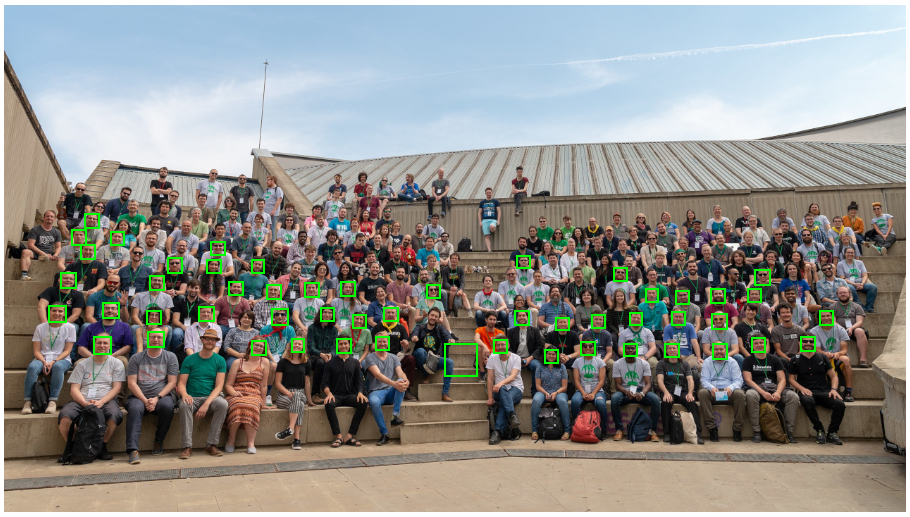
\includegraphics[width=0.85\textwidth]{Cap4_Experimentos_Realizados/Figures/cena1_param_720p_faces.jpg}
    \caption*{Fonte: autor.}
    \label{fig:otimizacaoCena1_720p}
\end{figure}

\begin{figure}
    \centering
    \caption[Tabela de Dados - resolução 720p.]{Tabela de Dados - resolução 720p.}
    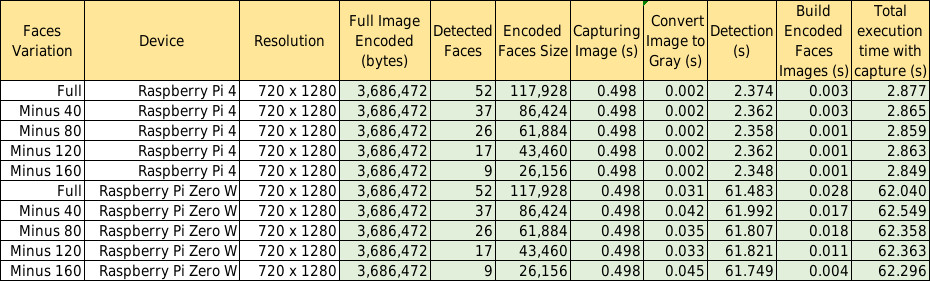
\includegraphics[width=0.90\textwidth]{Cap4_Experimentos_Realizados/Figures/cena1_dados_720p.jpg}
    \caption*{Fonte: autor.}
    \label{fig:dadosCena1_720p}
\end{figure}

\subsection{Análise dos resultados}
Nesta cena, são três fatores influenciando no resultado das detecções, seja quanto à capaidade de detecção e/ou quanto ao tempo de resposta. Esses fatores são a quantidade de faces detectáveis presentes na imagem, a resolução da imagem e o dispositivo rodando o algoritmo de detecção, sobre os quais serão feitas as comparações e análises a seguir.

\subsubsection{Efeitos da variação por quantidade de faces}

Os gráficos apresentados na figura \ref{fig:dadosCena1_graficos_variacao_faces} foram montados de forma a facilitar o entendimento de como a quantidade de faces influencia no tempo de detecção. Para maior clareza, os dados foram apresentados em três gráficos diferentes, um para cada resolução de imagem.
No eixo x, têm-se as variações de quantidade de faces detectáveis disponíveis. "Full" refere-se à imagem original, sem alteração, com todas as faces detectáveis, "Minus 40" refere-se à imagem trabalhada para borrar 40 faces de forma distribuída, tornando-as indetectáveis, e assim por diante.

Há três séries de dados cujas métricas são apresentadas para cada variação de faces. A quantidade de faces detectadas pelo algoritmo representada pelas barras verdes, que seguem a escala do eixo y à esquerda; o tempo total de execução nos testes com o Raspberry Pi 4B. em azul escuro, e o tempo total de execução nos teste com o Raspberry Pi Zero, em azul claro, ambos sguindo a escala do eixo y à direita, com unidade em segundos. Para melhor visualização, o eixo y à direita está em escala logarítmica.
O tempo de execução total é a soma do tempo de aquisição de imagem (nesse caso já considerando o tempo de captura do módulo câmera e não de leitura da imagem em arquivo), o tempo de conversão da imagem em escala de cinza, o tempo de detecção em si e o tempo de encodamento da imagem para transporte.
Há também a representação no gráfico, em linha amarela tracejada, do tempo de 5 segundos definido como limite para atender ao requisito da cena.

A ferramenta utilizada para a geração dos gráficos a partir da tebela de dados foi o \emph{Data Studio} \cite{DataStudio}, da Google.

Como se pode notar pela análise dos gráficos, a variação da quantidade de faces presentes, e por consequência detectadas, influencia muito pouco no tempo de detecção, chegando a 4\% a maior diferença. Observa-se esse comportamento em ambos os dispositvos testados e em todas a resoluções de imagem.

Com base nisso, pode-se dizer que, para a cena em questão, a quantidade de pessoas presentes no ambiente pouco no tempo de resposta do algoritmo em uso, o \textit{Haar cascade object detection} \cite{Viola2001}, podendo então este fator ser desconsiderado para quesitos de tempo (mas não de utilização de banda, obviamente).

\begin{figure}
    \centering
    \caption[Faces detectadas e Tempos de execução por Variação de faces detectáveis.]{Faces detectadas e Tempos de execução por Variação de faces detectáveis.}
    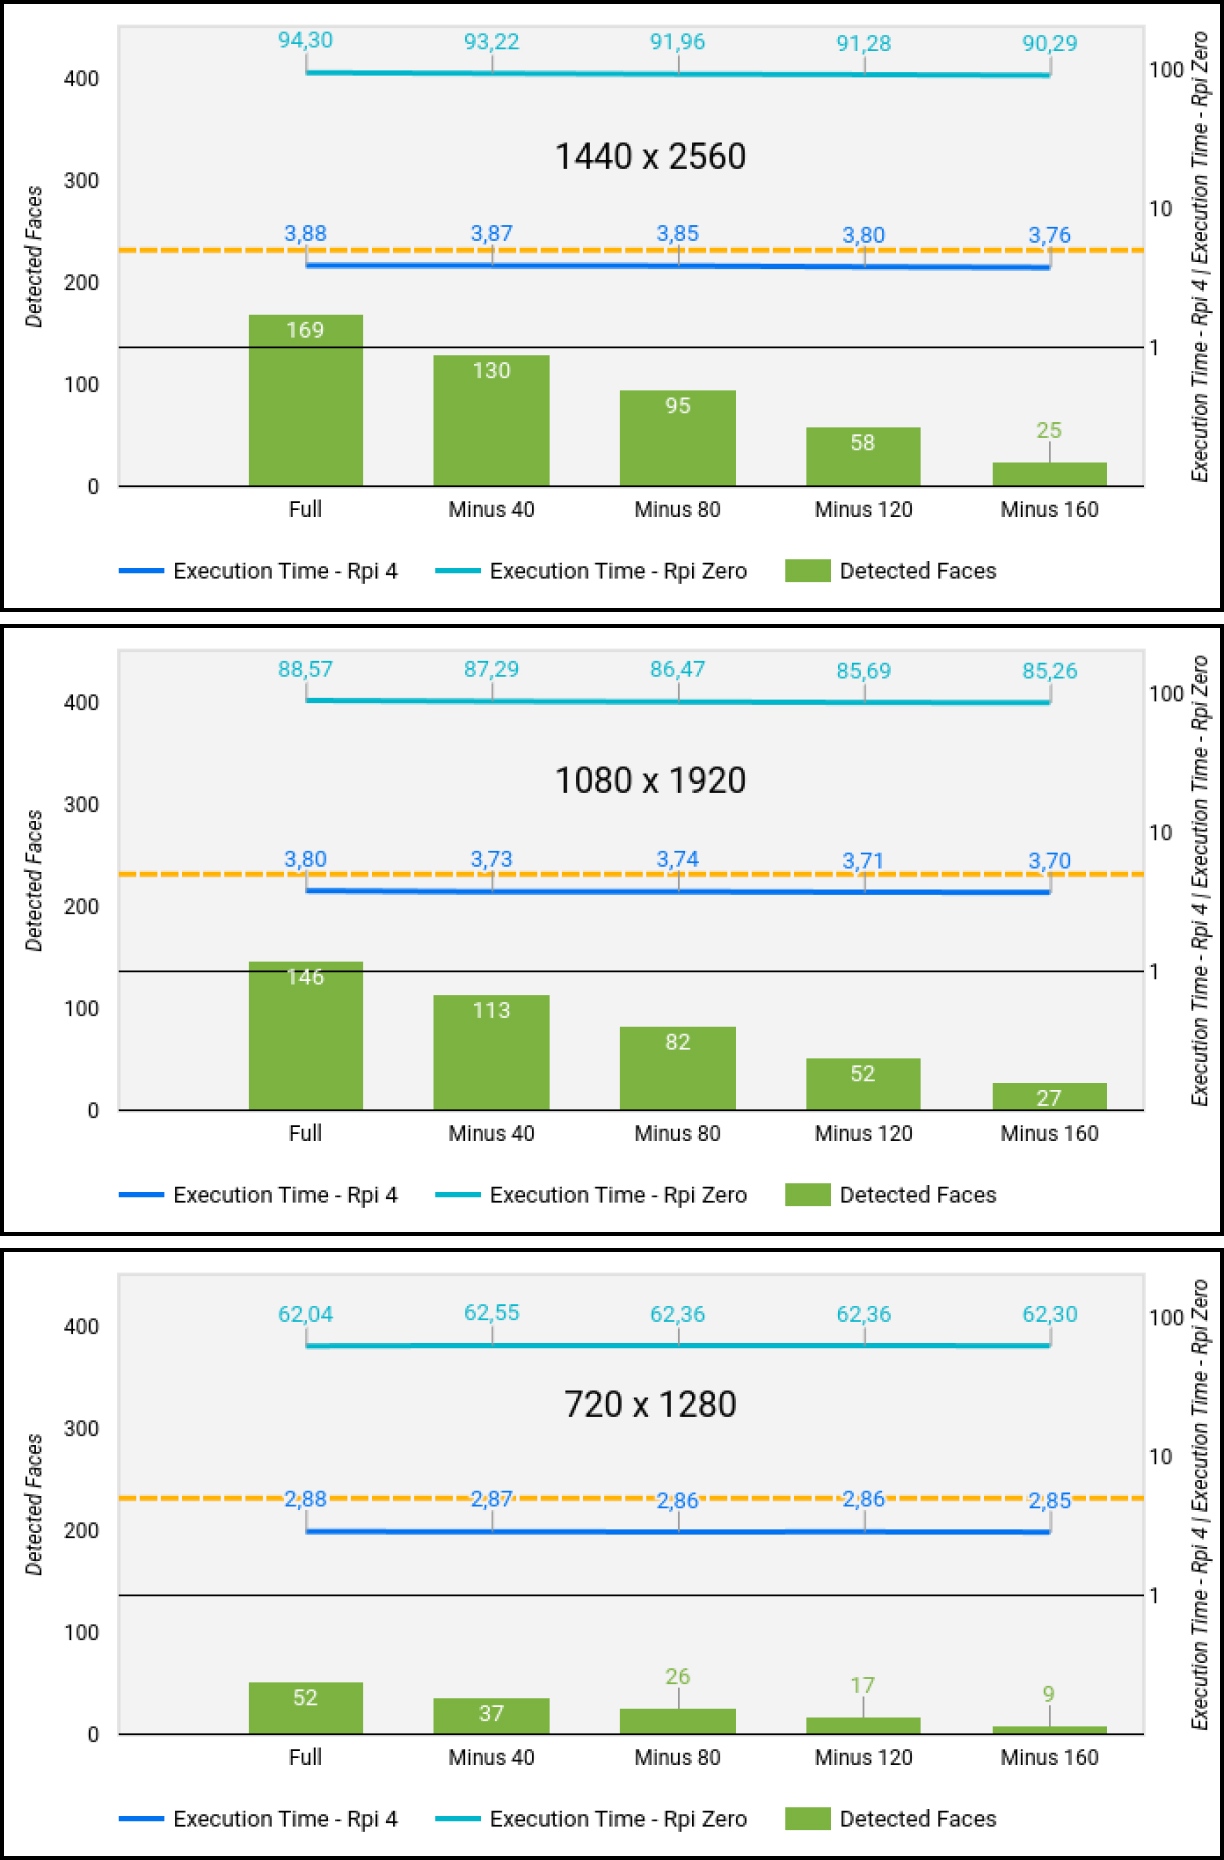
\includegraphics[width=0.7\textwidth]{Cap4_Experimentos_Realizados/Figures/cena1_graficos_variacao_faces.jpg}
    \caption*{Fonte: autor.}
    \label{fig:dadosCena1_graficos_variacao_faces}
\end{figure}

\subsubsection{Efeitos da variação por resolução de imagem}

Como foi constatado que a variação da quantidade de faces tem efeito insignificante no tempo de resposta, considerou-se apenas os resultados dos testes nas imagens com todas as faces detectáveis para montar o gráfico da figura \ref{fig:cena1_graficos_variacao_resolucao}, que têm a mesma estrutura dos gráficos anteriores, com a exceção de que no eixo x têm agora a variação por resolução de imagem.

Ao se comparar as duas maiores resoluções, 1440p e 1080p, observa-se que tanto o tempo de execução quanto o a quantidade de faces detectadas são menores na resolução menor, como é de se esperar. A redução no tempo é muito pouco expressiva, enquanto a redução na quantidade de faces detectadas não é tão expressiva mas pode-se considerar razoável.
Comparando-se as faces detectadas nessa duas resoluções, vide figuras \ref{fig:otimizacaoCena1_1440p} e \ref{fig:otimizacaoCena1_1080p}, percebe-se que as faces não detectadas são de pessoas que estão mais distantes na cena. Essa diferença de 25 faces (desconsiderando-se 2 falsos positivos na resolução de 1080p) pode ou não fazer grande diferença para a tomada de decisão, vai depender da realidade da cena real, se seria comum pessoas posicionadas tão distantes sem se aproximar da câmera, etc. 

É de se pensar que tendo menor resolução, a redução no tempo de resposta deveria ser razoavelmente menor devido à quantidade menor de pixels e quadros sendo processados. Porém, deve-se considerar também que, ao se buscar a maximização da quantidade de faces detectadas, reduziu-se o valor do parâmetro \emph{scale factor} durante a otimização, o que aumenta a quantidade de iterações no escalonamento. Comparando-se as matrizes de resultado nas figuras \ref{fig:otimizacaoCena1_1440p} e \ref{fig:otimizacaoCena1_1080p}, à medida que se caminha para a direita na matriz refente à resolução de 1080p, com valores maiores de \emph{scale factor} se aproximando ao selecionado para 1440p, observa-se uma redução considerável no tempo de detecção, com esperado, porém com também considerável redução na quantidade de faces detectadas.

Já comparando-se os resultados obtidos com a imagem de menor resolução, 720p, e as demais, a perda com relação à quantidade de faces detectadas é bastante expressiva, chegando a cair para menos de um terço da quantidade de faces detectadas na imagem de 1440p. Como pode ser visto na imagem \ref{fig:otimizacaoCena1_720p}, apenas as faces maiores (de pessoas mais próximas da câmera) são detectadas. A tempo de resposta tem uma queda até que razoável, porém não compensa a perda na quantidade de faces detectadas. Dessa forma, o uso de imagens com resolução de 720p se torna inadequado para o cenário em questão. 

\begin{figure}
    \centering
    \caption[Faces detectadas e Tempos de execução por Variação de resolução.]{Faces detectadas e Tempos de execução por Variação de resolução.}
    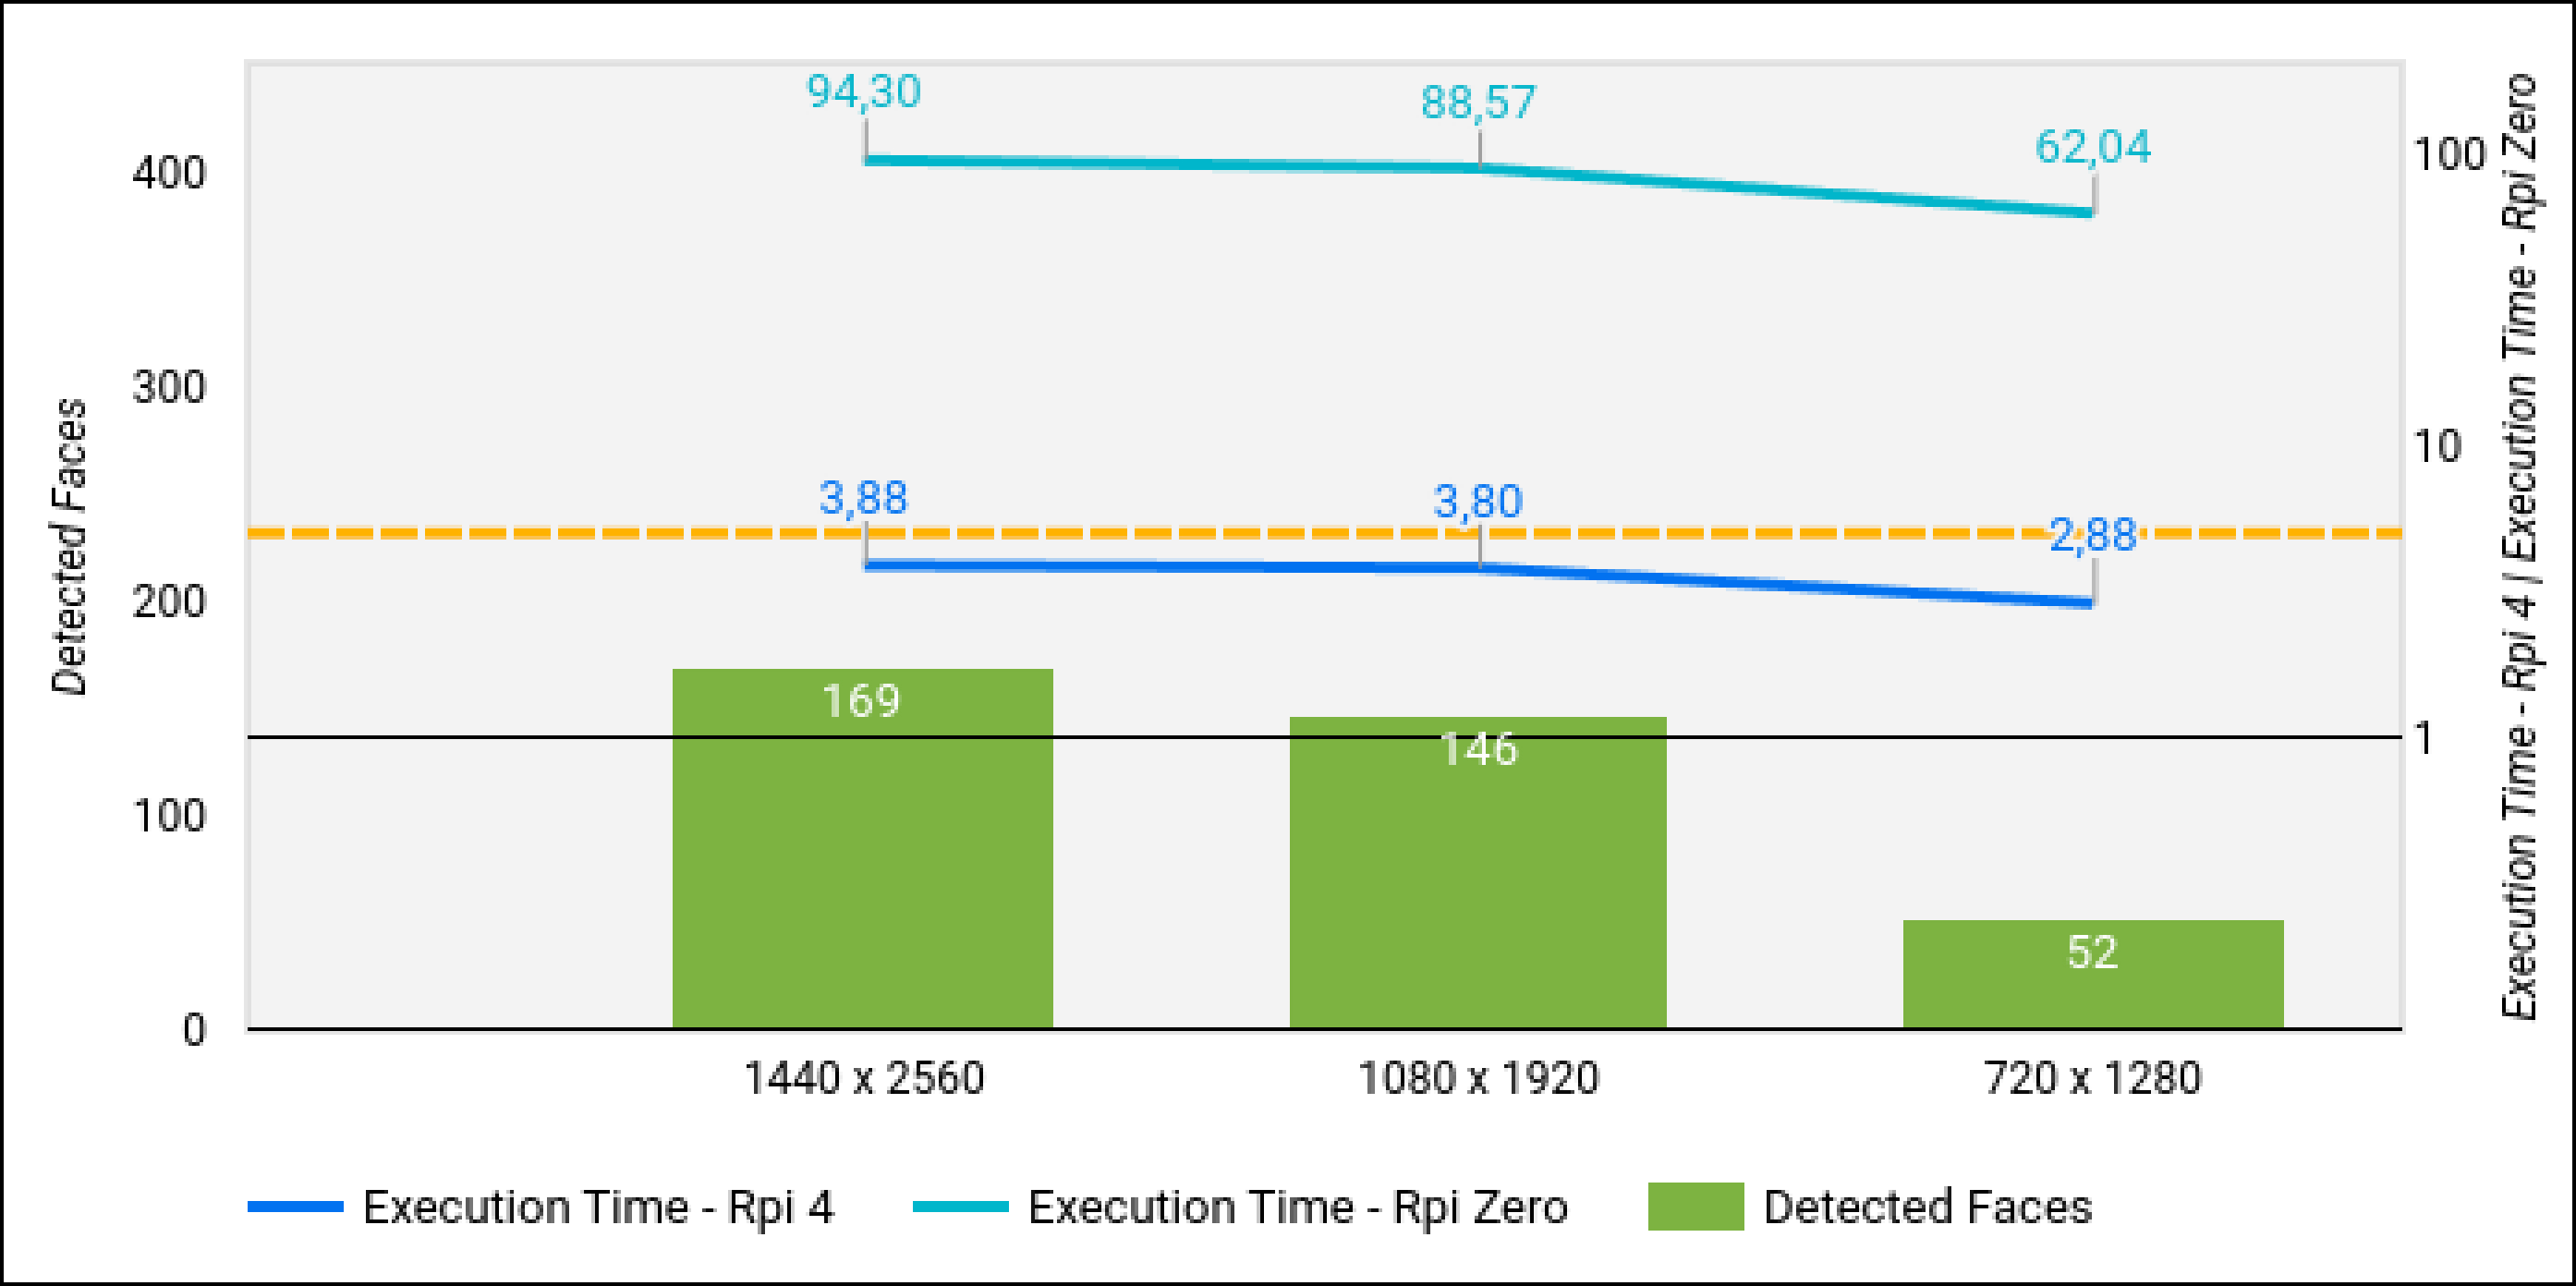
\includegraphics[width=0.7\textwidth]{Cap4_Experimentos_Realizados/Figures/cena1_graficos_variacao_resolucao.jpg}
    \caption*{Fonte: autor.}
    \label{fig:cena1_graficos_variacao_resolucao}
\end{figure}

Pode-se afirmar então que, a princípio, considerando-se apenas o \emph{trade-offf} entre quantidade de faces detectadas e tempo de resposta, a resolução de 1440p, a maior entre as  testadas, se mostra a mais adequada a se utilizar nesse tipo de cenário, onde objetiva-se detectar o máximo de faces possível e de tamanhos relativos muito pequenos.

Outra questão em que a utilização de resolução maior torna-se vantajoso é quanto à qualidade das imagens recortadas das faces. Caso as imagens das faces sejam utilizadas em uma próxima etapa da aplicação em outro disposivo na rede ou na nuvem, como por exemplo para reconhecimento facial ou simplesmente manter em registro, a qualidade e detalhes da face recortada pode fazer diferença no sucesso dessa próxima etapa.

Para se ter uma ideia mais visual da diferença, a figura \ref{fig:cena1_comparativo_qualidade_faces} faz um comparativo entre duas faces detectadas (a de uma pessoa mais próxima e a de uma pessoa mais distante) e as diferentes resoluções.


\begin{figure}
    \centering
    \caption[Comparativo de faces recortadas de deiferentes resoluções, em tamanho real.]{Comparativo de faces recortadas de deiferentes resoluções, em tamanho real.}
    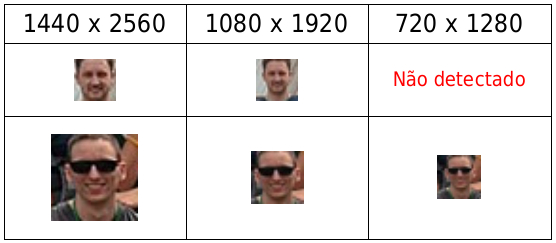
\includegraphics[width=0.8\textwidth]{Cap4_Experimentos_Realizados/Figures/cena1_comparativo_qualidade_faces_recortadas.jpg}
    \caption*{Fonte: autor.}
    \label{fig:cena1_comparativo_qualidade_faces}
\end{figure}

E o tamanho do dado que será trafegado (ver tamanho por face)

\subsubsection{Considerações sobre dispositivos}

\section{Cena 2}

\subsection{Captura de imagens para teste}

Conforme definido no capítulo anterior, as imagens para teste foram capturadas a partir de um módulo de câmera conectado no Raspbery Pi 4B.

A cena foi montada conforme pode ser visualizado na figura \ref{fig:cena2_posicao1_visao_externa}. O Raspberry Pi 4B, montado em sua case e com o módulo da câmera conectado foi fixado no batente lateral esquerdo da porta da entrada, de forma que a câmera ficasse posicionada a 1,7m do piso e levemente inclinada para baixo e para a dentro, na direção da passagem. A pessoa que aparece na imagem é o próprio autor.

Utilizando-se o script de captura de frames, foram feitos alguns testes e definiu-se essa como a posição mais próxima para se obter a primeira imagem a ser utilizada nos testes de desempenho, pois consegue pegar uma boa imagem do rosto e ainda com um pouco de folga vertical, considerando-se pessoas mais altas ou baixas.

\begin{figure}[H]
    \centering
    \caption[Posicionamento para captura da face na primeira posição.]{Posicionamento para captura da face na primeira posição.}
    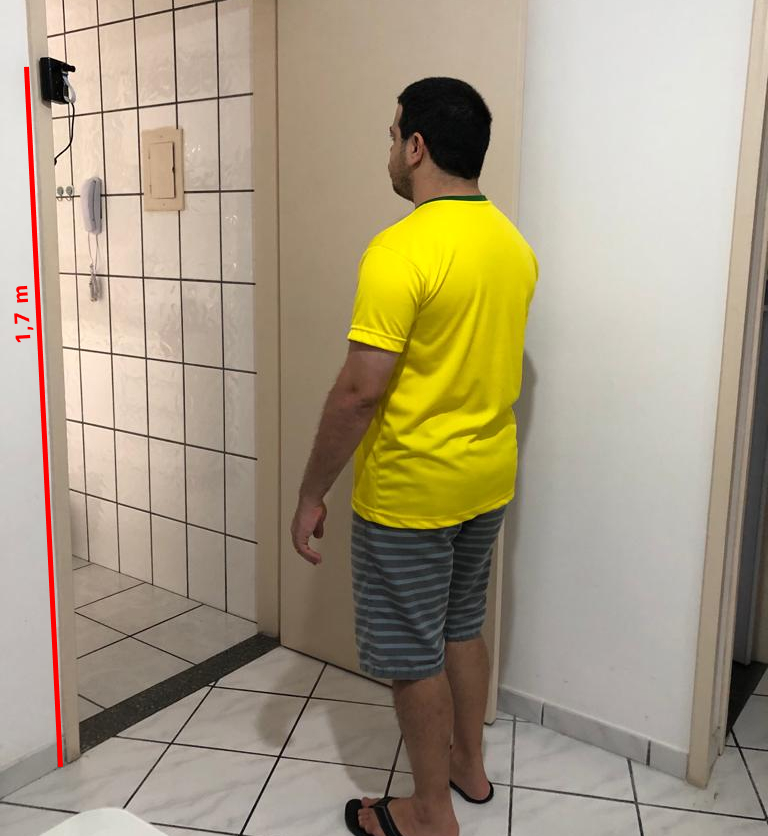
\includegraphics[width=0.65\textwidth]{Cap4_Experimentos_Realizados/Figures/cena2_posicao1_visao_externa.jpg}
    \caption*{Fonte: autor.}
    \label{fig:cena2_posicao1_visao_externa}
\end{figure}

Na figura \ref{fig:cena2_posicao1_imagem_capturada} têm-se a imagem capturada pela câmera na posição 1, na maior resolução definida para esta cena, 800x600.

\begin{figure}[H]
    \centering
    \caption[Captura da imagem na primeira posição.]{Captura da imagem na primeira posição.}
    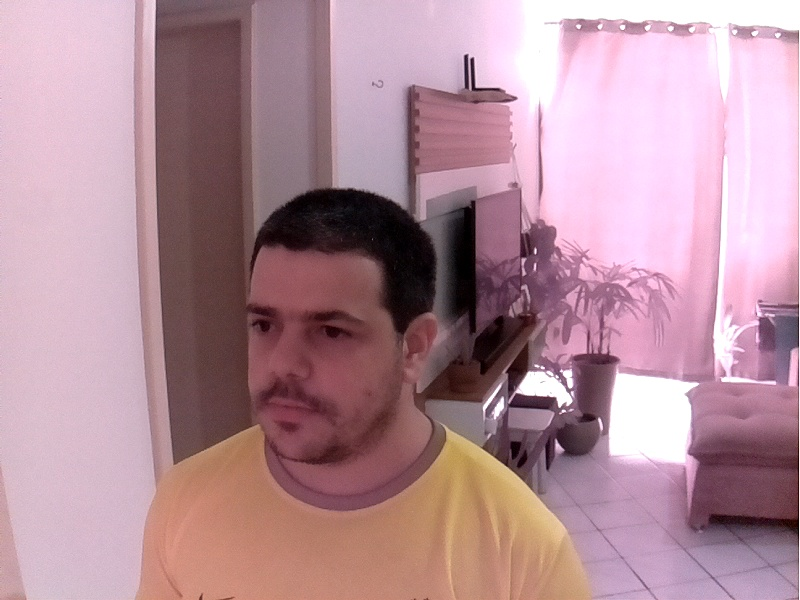
\includegraphics[width=0.65\textwidth]{Cap4_Experimentos_Realizados/Figures/cena2_posicao1_imagem_capturada.jpg}
    \caption*{Fonte: autor.}
    \label{fig:cena2_posicao1_imagem_capturada}
\end{figure}

A partir dessa primeira posição, mediu-se 1,7m distanciando-se da entrada. Essa é a posição mais distante, a partir da qual deseja-se que a face seja detectável. A figura \ref{fig:cena2_posicao2_visao_externa} demonstra esse posicionamento e na figura \ref{fig:cena2_posicao2_imagem_capturada} tem-se a imagem capturada pela câmera que também será utilizada nos testes.
\begin{figure}[H]
    \centering
    \caption[Posicionamento para captura da face na segunda posição.]{Posicionamento para captura da face na segunda posição.}
    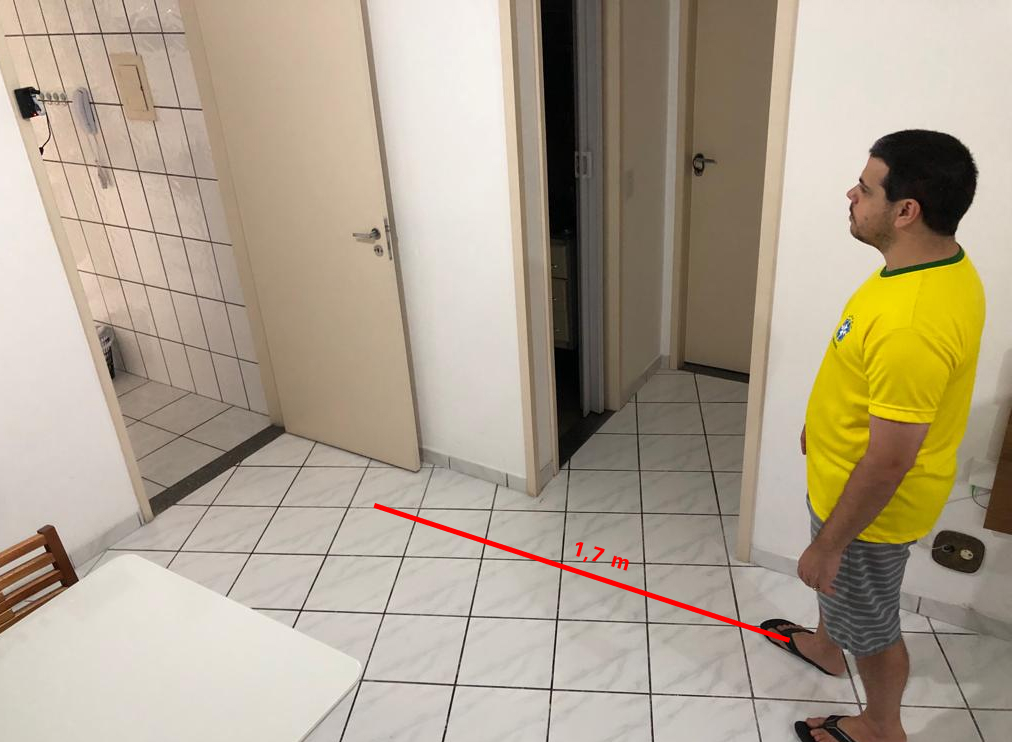
\includegraphics[width=0.65\textwidth]{Cap4_Experimentos_Realizados/Figures/cena2_posicao2_visao_externa.jpg}
    \caption*{Fonte: autor.}
    \label{fig:cena2_posicao2_visao_externa}
\end{figure}

\begin{figure}[H]
    \centering
    \caption[Captura da imagem na segunda posição.]{Captura da imagem na segunda posição.}
    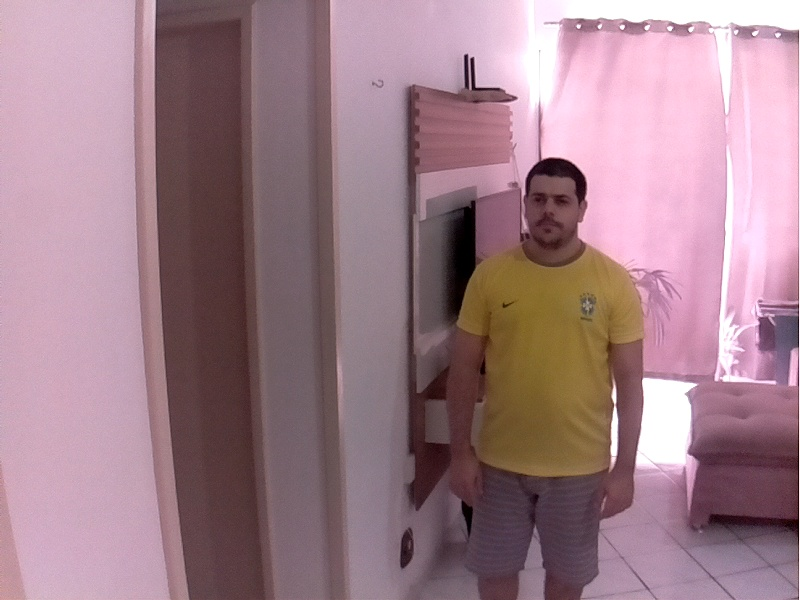
\includegraphics[width=0.65\textwidth]{Cap4_Experimentos_Realizados/Figures/cena2_posicao2_imagem_capturada.jpg}
    \caption*{Fonte: autor.}
    \label{fig:cena2_posicao2_imagem_capturada}
\end{figure}


\subsection{Otimização de parâmetros}

Foi realizada a otimização dos parâmetros para cada variação de resolução, utilizando-se as imagens capturadas nas duas posições. Utilizou-se o Raspberry Pi 4B para a definição dos parâmetros, repetindo-os nos testes com o Raspberry Pi Zero W para base de comparação.

As imagens em ambas as posições foram analisadas em conjunto mas com o objetivo de se chegar a apenas um conjunto de parâmetros 'ótimos' para obtenção das métricas. Foram considerados 'ótimos' a mesma combinação de parâmetros que atendia as duas imagens, buscando-se os limiares com o menor tempo em que as faces são detectadas e sem falsos positivos. Para facilitar a visualização desses limiares, foram definidos passos maiores de ScaleFactor e Min. Size para se obter quantidades maiores de amostras.

Pode-se pensar, a princípio, que bastava analisar a imagem na posição 2, que é a mais distante, pois essa já seria o pior caso, já que a face teria menor resolução que a da posição 1. Porém, percebe-se claramente comparando as figuras \ref{fig:cena2_posicao1_imagem_capturada} e \ref{fig:cena2_posicao2_imagem_capturada} que quando a face está mais próxima da câmera e estando a pessoa olhando naturalmente em direção à entrada, o angulo não é muito bom, podendo criar alguma dificuldade adicional na detecção da face. Por isso a importância da análise conjunta.

Para se considerar um pior caso, foram utilizados os dados das métricas que apresentaram maiores tempos de resposta e tamanho de imagem, isso para cada resolução.

As próximas três subsubseções \ref{sssec:resolution2-1}, \ref{sssec:resolution2-2} e \ref{sssec:resolution2-3} mostram para cada resolução testada, a última iteração da matriz de resultados para a detecção em ambas as posições, com os dados entrada, a célula destacada com os parâmetros escolhidos e as imagems com a faces detectadas. Nas figuras das matrizes foram adicionadas linhas azuis (para a posição 1) e vermelhas (para aposição 2), indicando limiares que separam os grupos contínuos de resultados onde há detecção de face. Foram então selecionados os melhores resultados dentro da interseção desses grupos .

Após os parâmetros definidos no Raspberry Pi 4, os mesmos foram utilizados para obter a métricas no Raspberry Pi Zero W, sendo todos tabelados para comparação.


\subsubsection{Resolução 600p} \label{sssec:resolution2-1}

Devido ao tamanho maior das matrizes de resultados e a necessidade de visualização lado à lado, a parte da interface com os controles de parametrização não foram exibidos. Os prâmetros utilizados foram: "Min. Neighbors: 3", "Number of Samples: 6". Início e fim de escala dos demais parâmetros podem ser vistos nas matrizes.



\begin{figure}[H]
    \centering
    \caption[Otimização Cena 2 - resolução 600p - matrizes. À esquerda posição 1 e à direita, posição 2]{Otimização Cena 2 - resolução 600p - matrizes. À esquerda, posição 1, e à direita, posição 2.}
    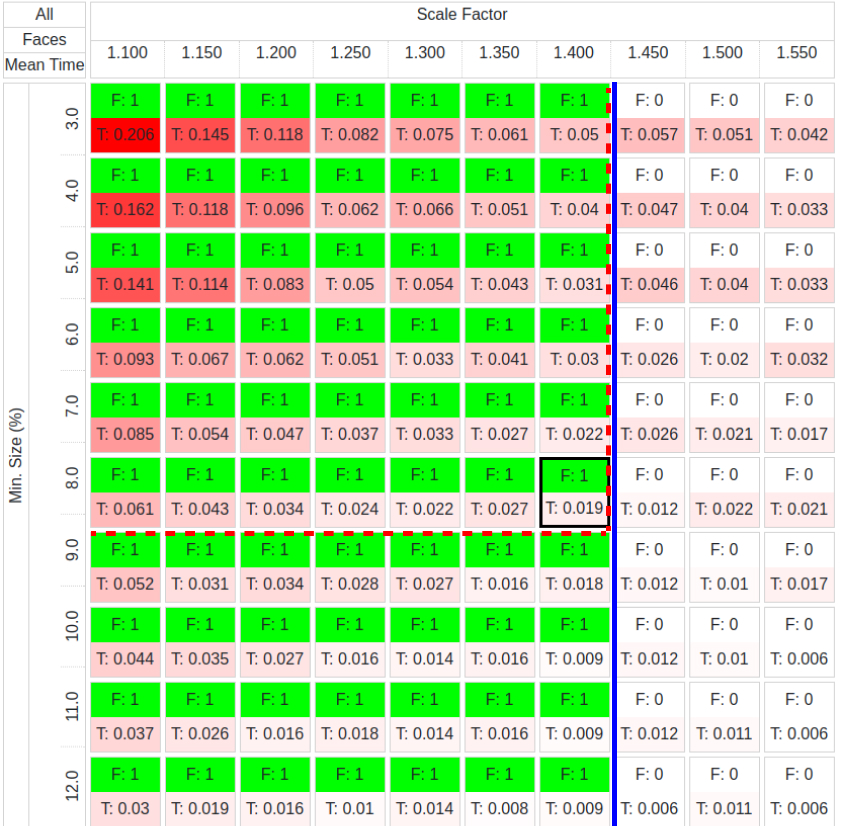
\includegraphics[width=0.49\textwidth]{Cap4_Experimentos_Realizados/Figures/cena2_800x600_pos1_matriz.jpg}
    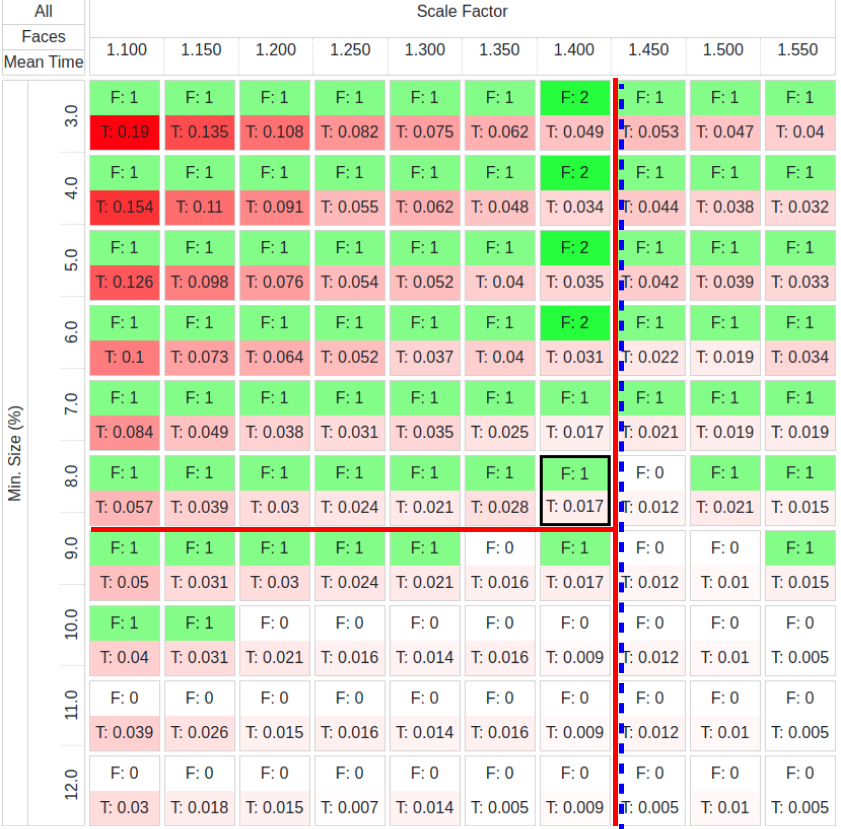
\includegraphics[width=0.49\textwidth]{Cap4_Experimentos_Realizados/Figures/cena2_800x600_pos2_matriz.jpg}
    \caption*{Fonte: autor.}
    \label{fig:otimizacaoCena2_600p_matrizes}
\end{figure}

\begin{figure}[H]
    \centering
    \caption[Otimização Cena 2 - resolução 600p - face detectada. À esquerda posição 1 e à direita, posição 2]{Otimização Cena 2 - resolução 600p - face detectada. À esquerda, posição 1, e à direita, posição 2.}
    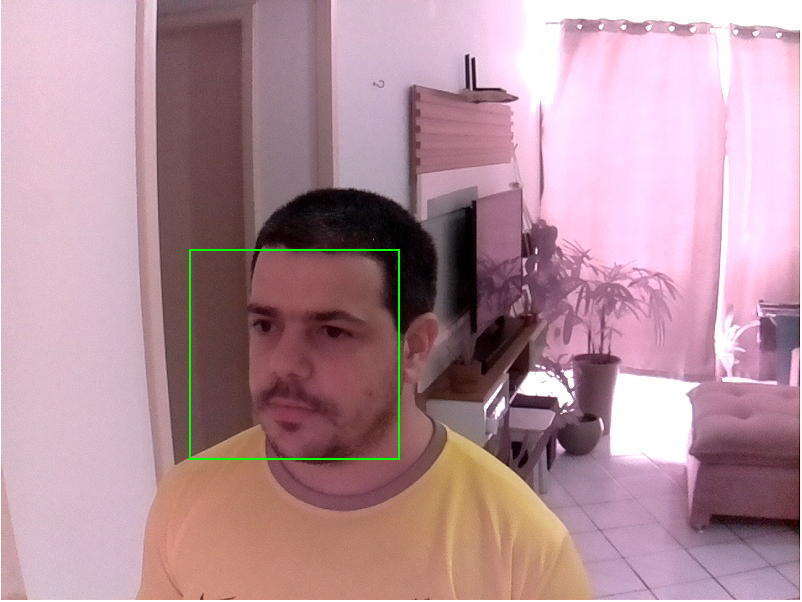
\includegraphics[width=0.49\textwidth]{Cap4_Experimentos_Realizados/Figures/cena2_800x600_pos1_face.jpg}
    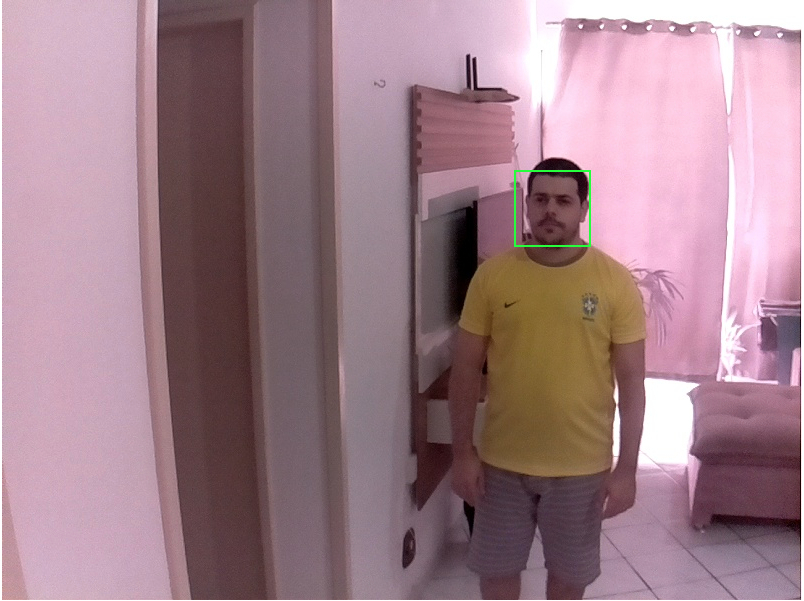
\includegraphics[width=0.49\textwidth]{Cap4_Experimentos_Realizados/Figures/cena2_800x600_pos2_face.jpg}
    \caption*{Fonte: autor.}
    \label{fig:otimizacaoCena2_600p_faces}
\end{figure}

\subsubsection{Resolução 480p} \label{sssec:resolution2-2}

\begin{figure}[H]
    \centering
    \caption[Otimização Cena 2 - resolução 480p - matrizes. À esquerda posição 1 e à direita, posição 2]{Otimização Cena 2 - resolução 480p - matrizes. À esquerda, posição 1, e à direita, posição 2.}
    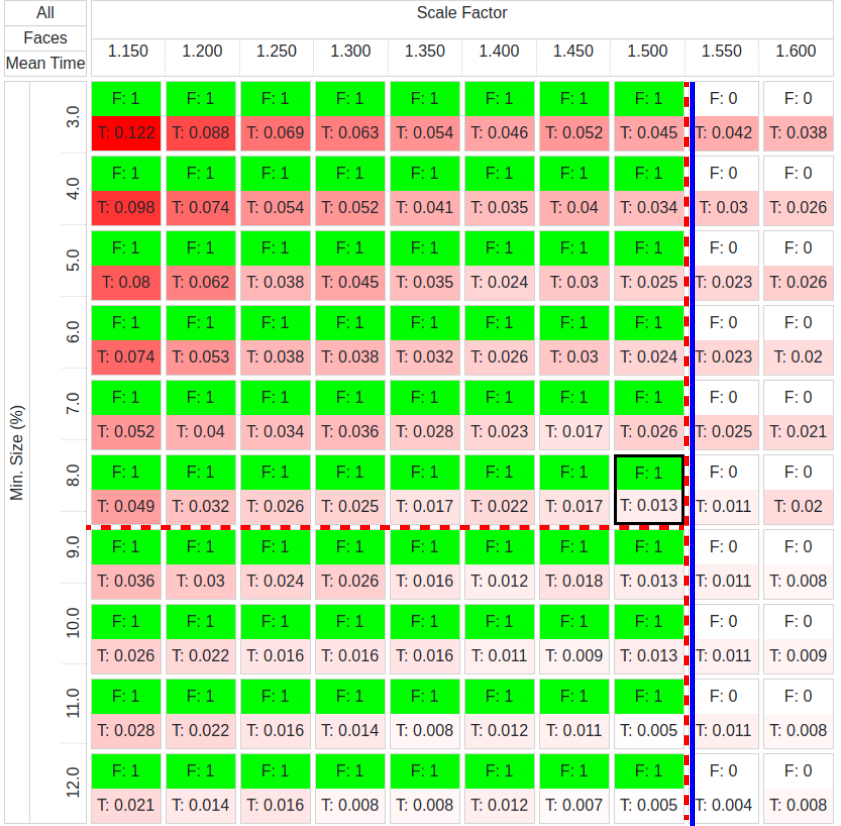
\includegraphics[width=0.49\textwidth]{Cap4_Experimentos_Realizados/Figures/cena2_640x480_pos1_matriz.jpg}
    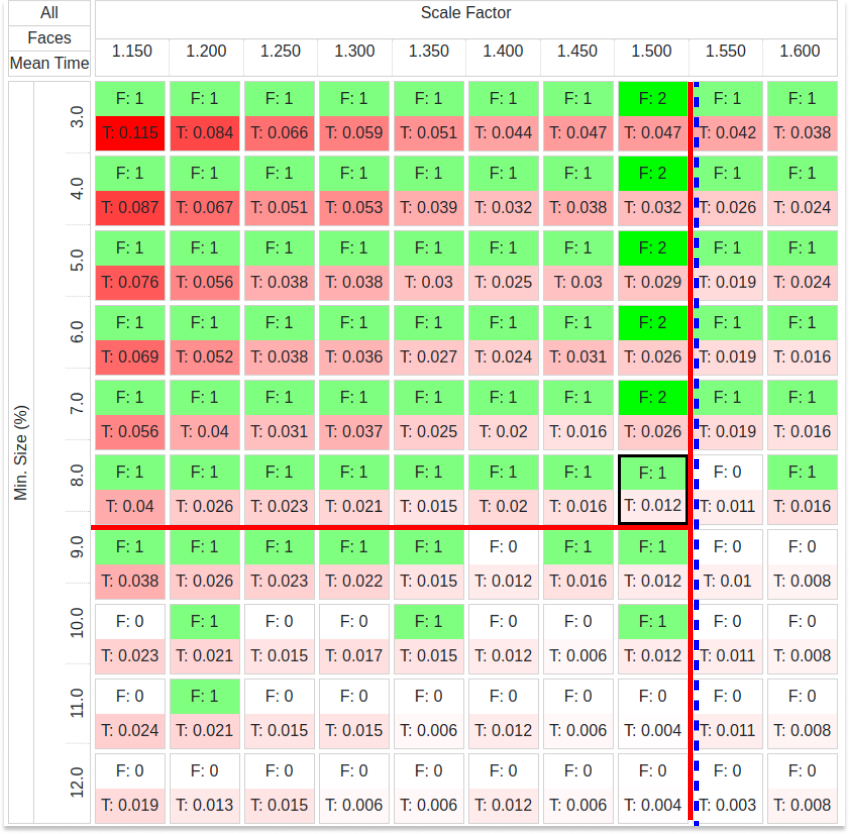
\includegraphics[width=0.49\textwidth]{Cap4_Experimentos_Realizados/Figures/cena2_640x480_pos2_matriz.jpg}
    \caption*{Fonte: autor.}
    \label{fig:otimizacaoCena2_480p_matrizes}
\end{figure}

\begin{figure}[H]
    \centering
    \caption[Otimização Cena 2 - resolução 480p - face detectada. À esquerda posição 1 e à direita, posição 2]{Otimização Cena 2 - resolução 480p - face detectada. À esquerda, posição 1, e à direita, posição 2.}
    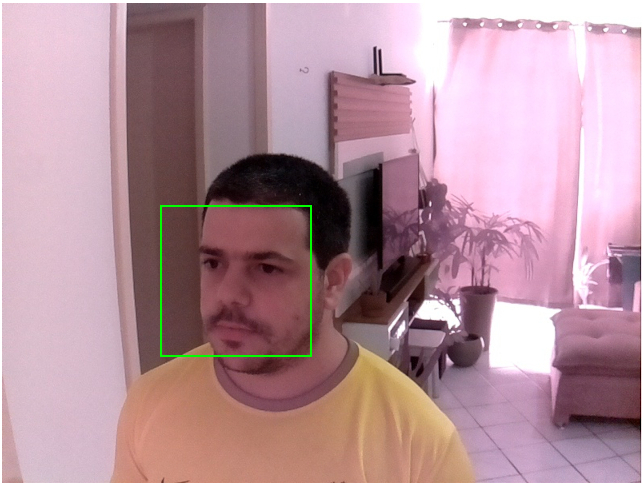
\includegraphics[width=0.49\textwidth]{Cap4_Experimentos_Realizados/Figures/cena2_640x480_pos1_face.jpg}
    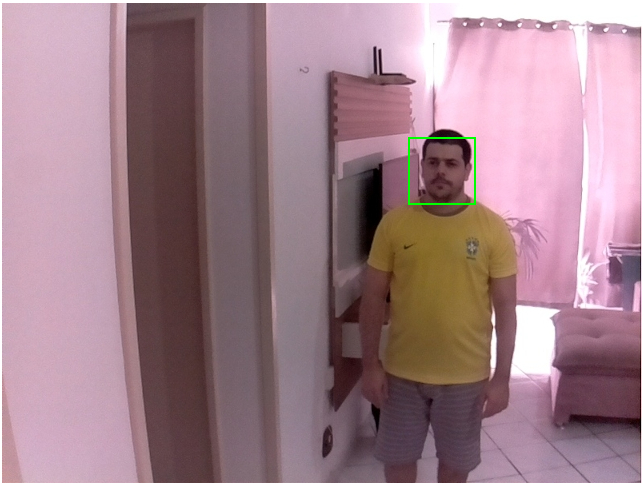
\includegraphics[width=0.49\textwidth]{Cap4_Experimentos_Realizados/Figures/cena2_640x480_pos2_face.jpg}
    \caption*{Fonte: autor.}
    \label{fig:otimizacaoCena2_480p_faces}
\end{figure}

\subsubsection{Resolução 240p} \label{sssec:resolution2-3}

\begin{figure}[H]
    \centering
    \caption[Otimização Cena 2 - resolução 240p - matrizes. À esquerda posição 1 e à direita, posição 2]{Otimização Cena 2 - resolução 240p - matrizes. À esquerda, posição 1, e à direita, posição 2.}
    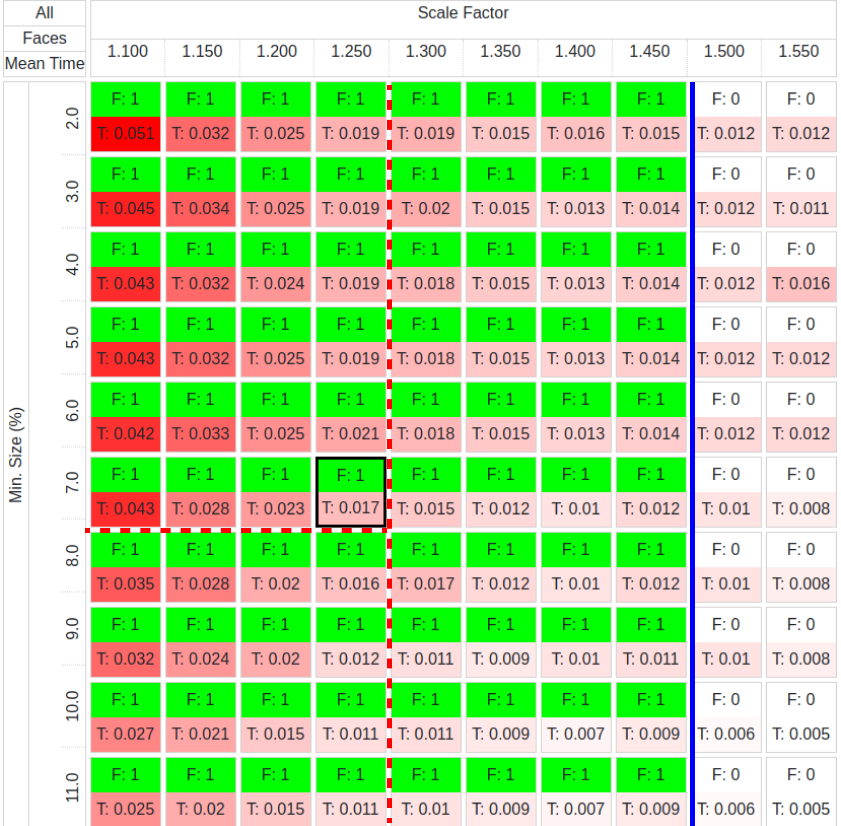
\includegraphics[width=0.49\textwidth]{Cap4_Experimentos_Realizados/Figures/cena2_320x240_pos1_matriz.jpg}
    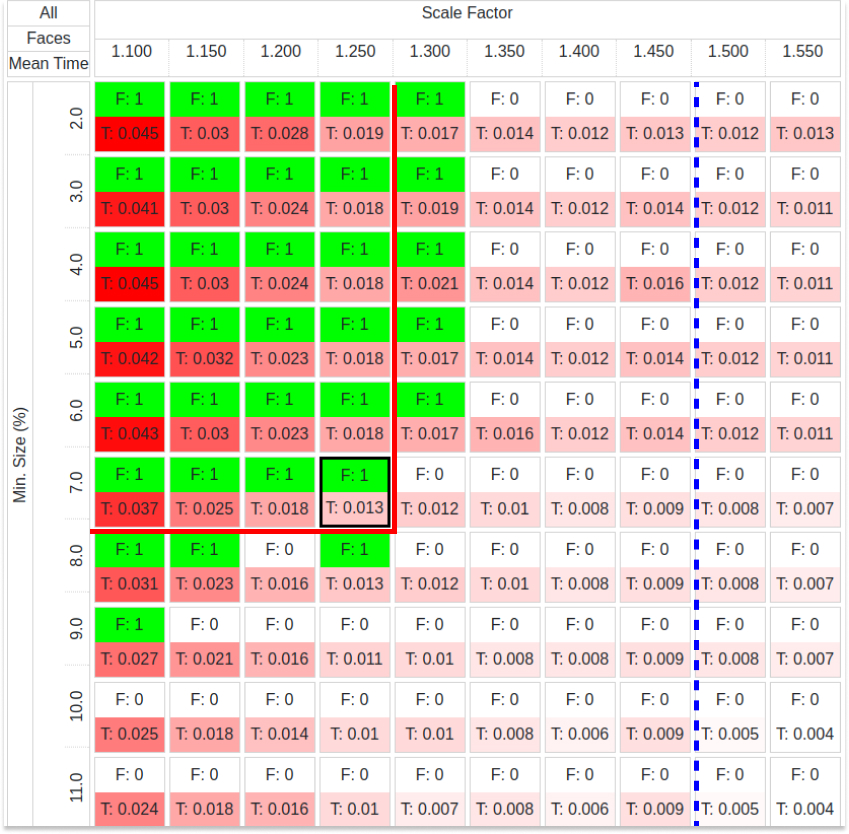
\includegraphics[width=0.49\textwidth]{Cap4_Experimentos_Realizados/Figures/cena2_320x240_pos2_matriz.jpg}
    \caption*{Fonte: autor.}
    \label{fig:otimizacaoCena2_240p_matrizes}
\end{figure}

\begin{figure}[H]
    \centering
    \caption[Otimização Cena 2 - resolução 240p - face detectada. À esquerda posição 1 e à direita, posição 2]{Otimização Cena 2 - resolução 240p - face detectada. À esquerda, posição 1, e à direita, posição 2.}
    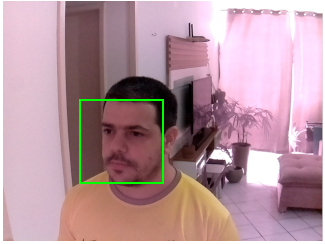
\includegraphics[width=0.49\textwidth]{Cap4_Experimentos_Realizados/Figures/cena2_320x240_pos1_face.jpg}
    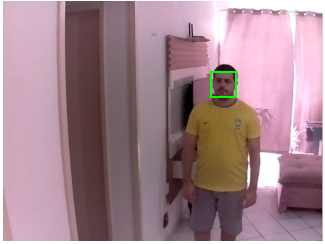
\includegraphics[width=0.49\textwidth]{Cap4_Experimentos_Realizados/Figures/cena2_320x240_pos2_face.jpg}
    \caption*{Fonte: autor.}
    \label{fig:otimizacaoCena2_240p_faces}
\end{figure}

- colocar as imagens das faces cortadas em tamanho real para demonstração
- ver se incluo de alguma forma os dados da métricas para cada resolução testada



lembretes para discussão:

cena 2
- no rpi4 todos atendem e qaunto menos resolução mais rápido, porém menos qualidade. Talvez faça sentido usar resolução mais alta para ter mais qualidade na frente como em algum reconhecimento de face
- no RpiZ não atende. Talvez possa ser usado para reconhecimento mais proximo como identificação de face para liberação de acesso com a face parada por mais tempo na frente, poderia-se at´e utilizar resolução menor, etc Coisa que pode entrar em trabalhos futuros tabelados

- Tempo de captura relativamente grande. Possibilidade de melhorar tempo total com threads separadas e ou outras formas de captura, etc. (tb possivel em trabalhos futuros)